% !TEX root = ../../main.tex
\section{Data Gathering}\label{sec:data_gathering}
For our data sets of real world activities we have sampled both in- and outdoor activites.
The subjects performing the activities are three males, in an age around 25.
We have used two series of recordings.
The first series are various outdoor recordings with segments of walking, running and standing.
Some movement activities are performed in a straight line, whilst others are performed around corners of in a wide circular direction.
The second series consist of mainly walking up and down the stairs, with small vertical parts between the segments.
The stairs are all in a circular shape.

\subsection{Outside}\label{subsec:outside}

\TODO{For each data set: discovered timepoint with acc, mag, rot, and all combined. Use closest change point}

\begin{center}\begin{table}
  \begin{tabulary}{\textwidth}{|c|c|c|}
    \hline
    \multicolumn{3}{|c|}{Subj 1, run 1} \\
    \hline \hline
    Act. & Ann. & Disc. \\
    \hline
    Still & 0 & *0* \\
    \hline
    Shake & 3.5 & *3.5* \\
    \hline
    Still & 4.2 & *4.2* \\
    \hline
    In pocket & 5.5 & *5.5* \\
    \hline
    Walk & 7 & *7* \\
    \hline
    Run & 10 & *10* \\
    \hline
    Walk & 14 & *14* \\
    \hline
    Run & 17.2 & *17.2* \\
    \hline
    Walk & 22.1 & *22.1* \\
    \hline
    Turn CCW & 23.5 & *23.5* \\
    \hline
    Walk & 24.2 & *24.2* \\
    \hline
    Run (sprint) & 28 & *28* \\
    \hline
    Run & 31 & *31* \\
    \hline
    Walk & 33 & *33* \\
    \hline
    Run & 35.5 & *35.5* \\
    \hline
    Walk & 39 & *39* \\
    \hline
    Out pocket & 41 & *41* \\
    \hline
    Still & 43 & *43* \\
    \hline
  \end{tabulary}
  \caption[Performed activities subject 1 run 1]{The outdoor series performed activities by subject 1, run 1.}
  \label{tab:outdoor_series}
\end{table}\end{center}

\begin{center}\begin{table}
  \begin{tabulary}{\textwidth}{|c|c|c|}
    \hline
    \multicolumn{3}{|c|}{Subj 2, run 1} \\
    \hline \hline
    Act. & Ann. & Disc. \\
    \hline
    Still & 0 & *0* \\
    \hline
    Shake & 4 & *4* \\
    \hline
    Still & 5 & *5* \\
    \hline
    In pocket & 8.8 & *8.8* \\
    \hline
    Walk & 12 & *12* \\
    \hline
    Run & 16 & *16* \\
    \hline
    Walk & 21.3 & *21.3* \\
    \hline
    Run & 24.5 & *24.5* \\
    \hline
    Walk & 28.3 & *28.3* \\
    \hline
    Turn CCW & 30 & *30* \\
    \hline
    Walk & 31.8 & *31.8* \\
    \hline
    Run & 32.8 & *32.8* \\
    \hline
    Walk & 37 & *37* \\
    \hline
    Run (sprint) & 39.5 & *39.5* \\
    \hline
    Run & 42 & *42* \\
    \hline
    Walk & 44.5 & *44.5* \\
    \hline
    Out pocket & 49.5 & *49.5* \\
    \hline
    Still & 52 & *52* \\
    \hline
    Shake & 55.7 & *55.7* \\
    \hline
    Still & 56.8 & *56.8* \\
    \hline
  \end{tabulary}
  \caption[Performed activities subject 2 run 1]{The outdoor series performed activities by subject 2, run 1.}
  \label{tab:outdoor_series}
\end{table}\end{center}

\TODO{Replace all times in the stars with the closest discovered change point}

%---- Run 1: walk-run-roemer
\begin{figure}
\centering
  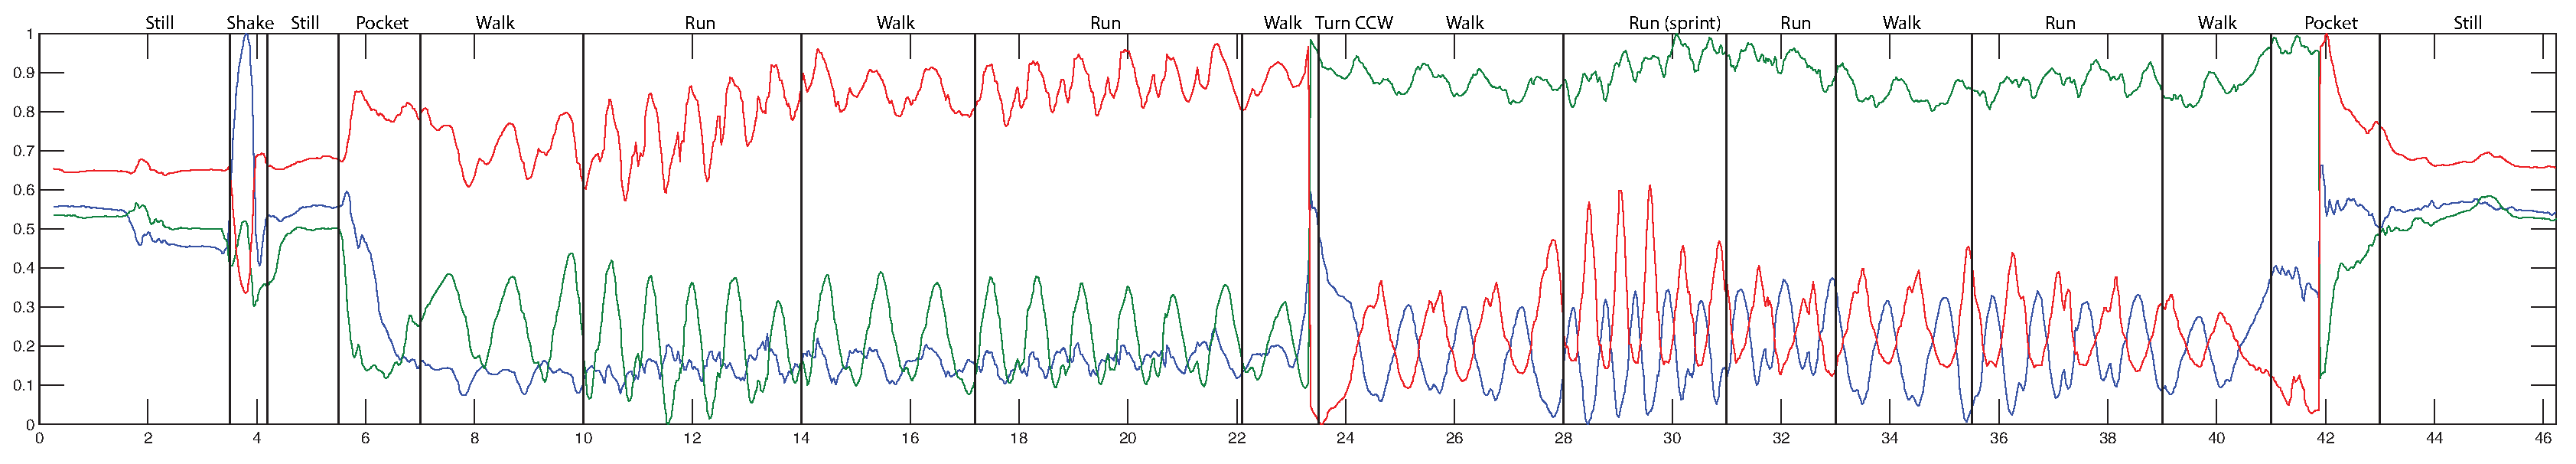
\includegraphics[width=1\textwidth]{./Figures/chapter6/data_collection/run-1-walk-run-roemer/data_plot_rot_annotated.eps}
  \caption[R1: rotation]{Run 1: Walk-run-roemer, rotation}
  \label{fig:data_gathering_run_1_rot}
\end{figure}

\begin{figure}
\centering
  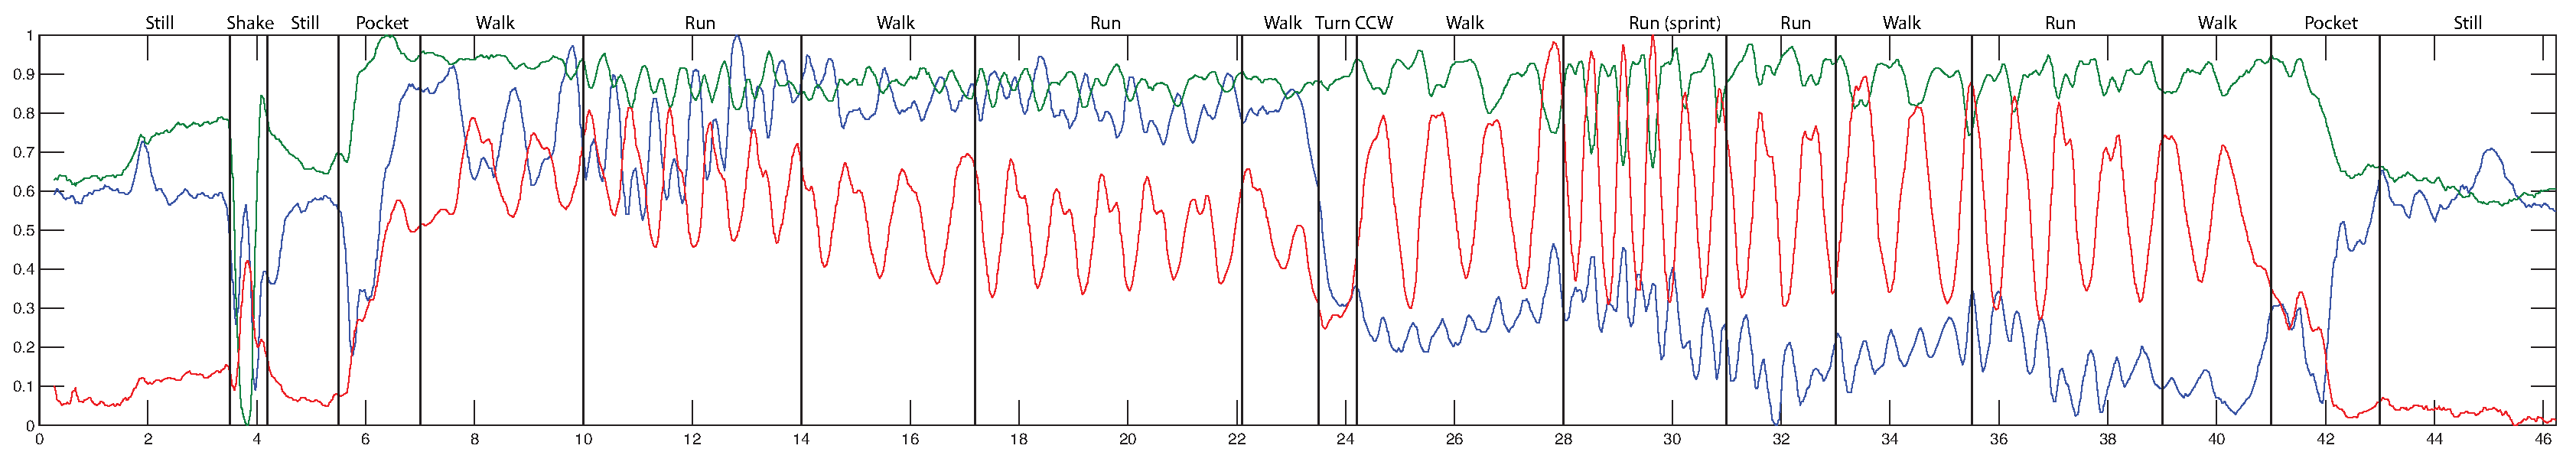
\includegraphics[width=1\textwidth]{./Figures/chapter6/data_collection/run-1-walk-run-roemer/data_plot_mag_annotated.eps}
  \caption[R1: mag]{Run 1: Walk-run-roemer, Mag}
  \label{fig:data_gathering_run_1_mag}
\end{figure}

\begin{figure}
\centering
  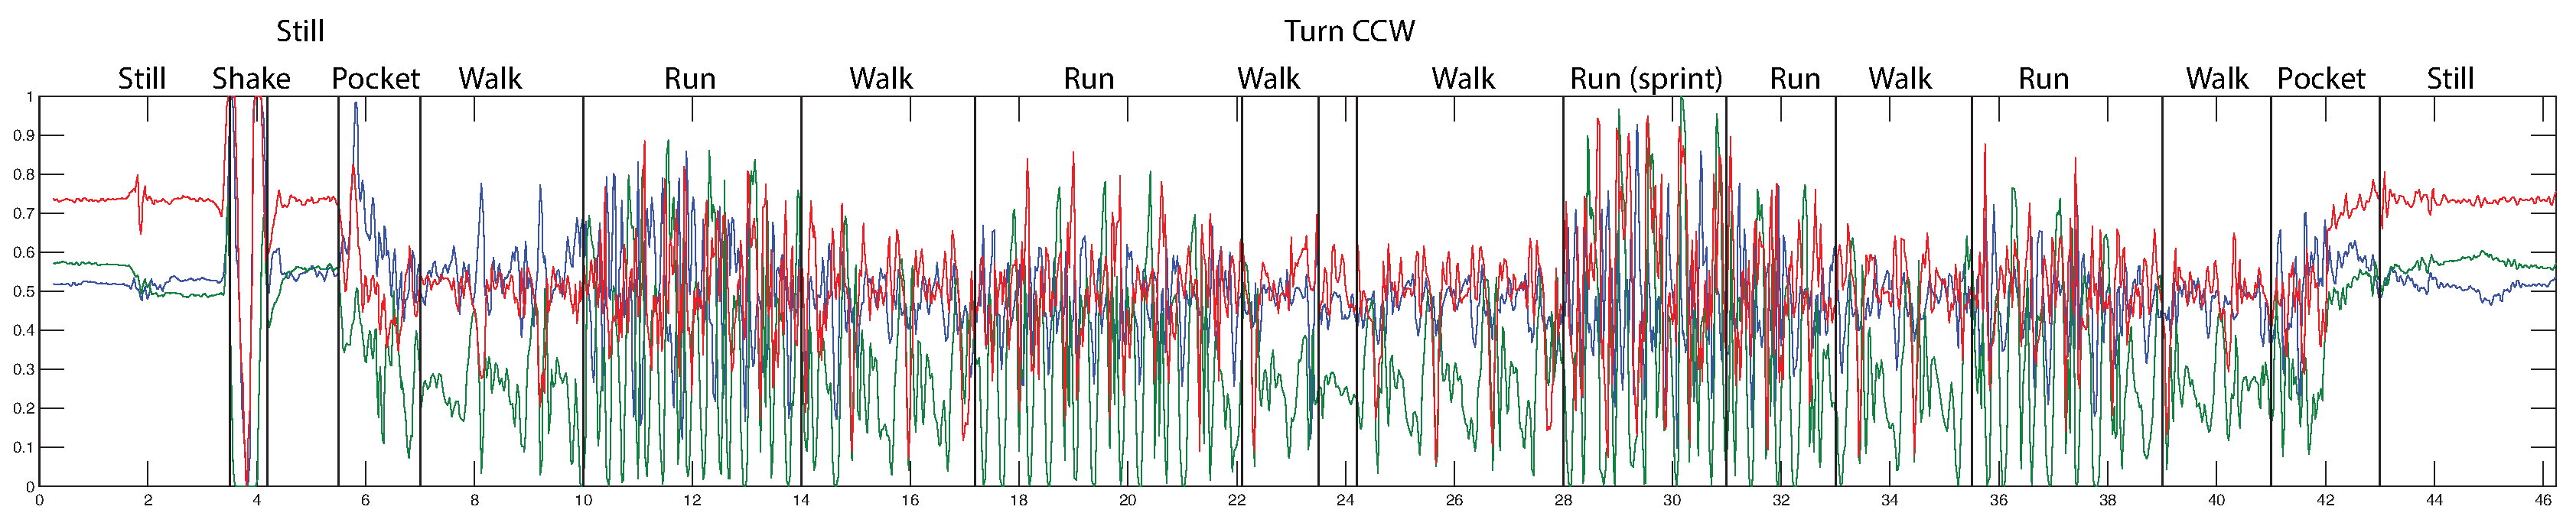
\includegraphics[width=1\textwidth]{./Figures/chapter6/data_collection/run-1-walk-run-roemer/data_plot_acc_annotated.eps}
  \caption[R1: accelerometer]{Run 1: Walk-run-roemer, accelerometer}
  \label{fig:data_gathering_run_1_ann}
\end{figure}

%---- Run 2: walk-run-jos
\begin{figure}
\centering
  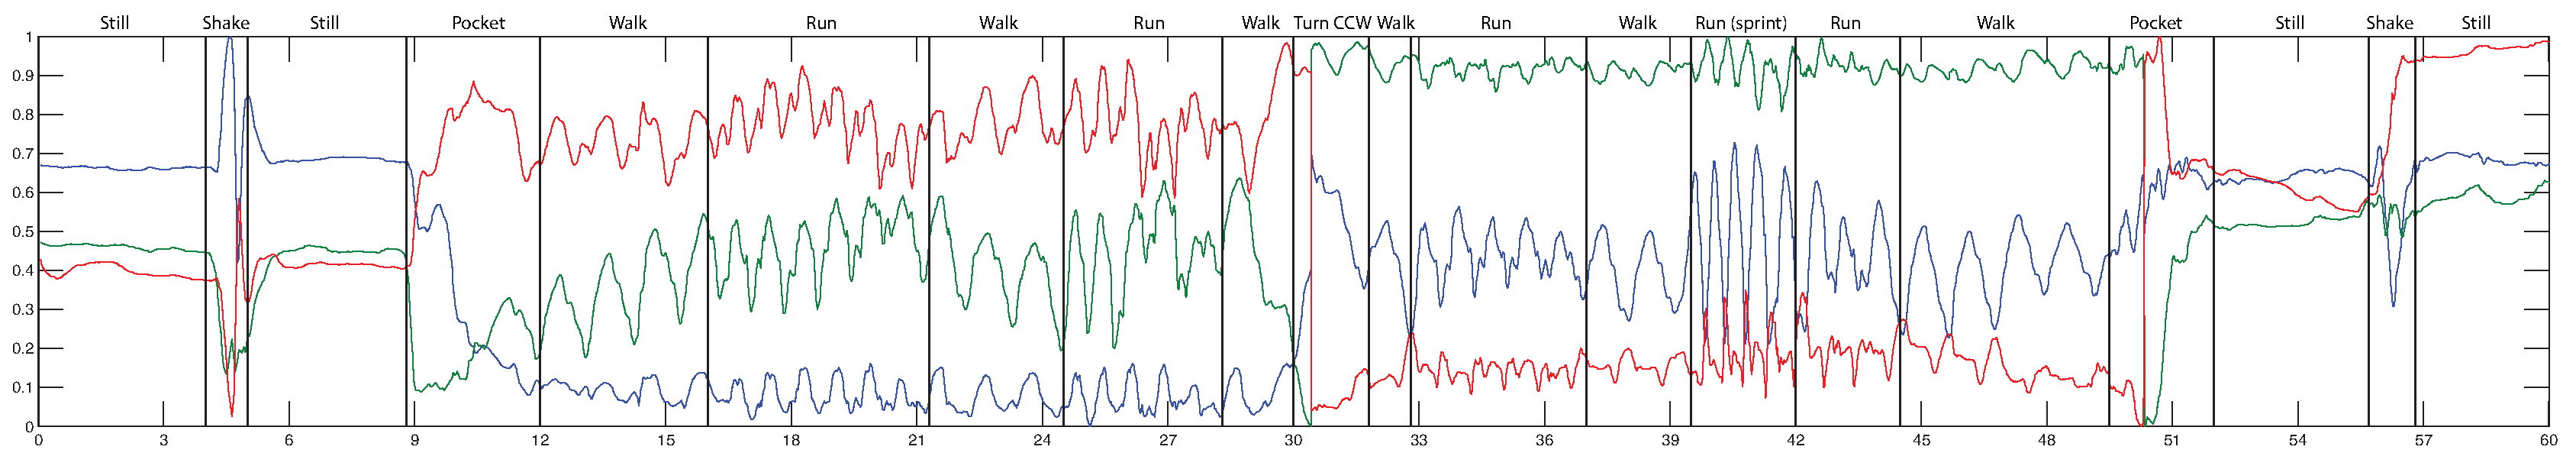
\includegraphics[width=1\textwidth]{./Figures/chapter6/data_collection/run-2-walk-run-jos/data_plot_rot_annotated.eps}
  \caption[R2: rotation]{Run 2: Walk-run-jos, rotation}
  \label{fig:data_gathering_run_2_rot}
\end{figure}

\begin{figure}
\centering
  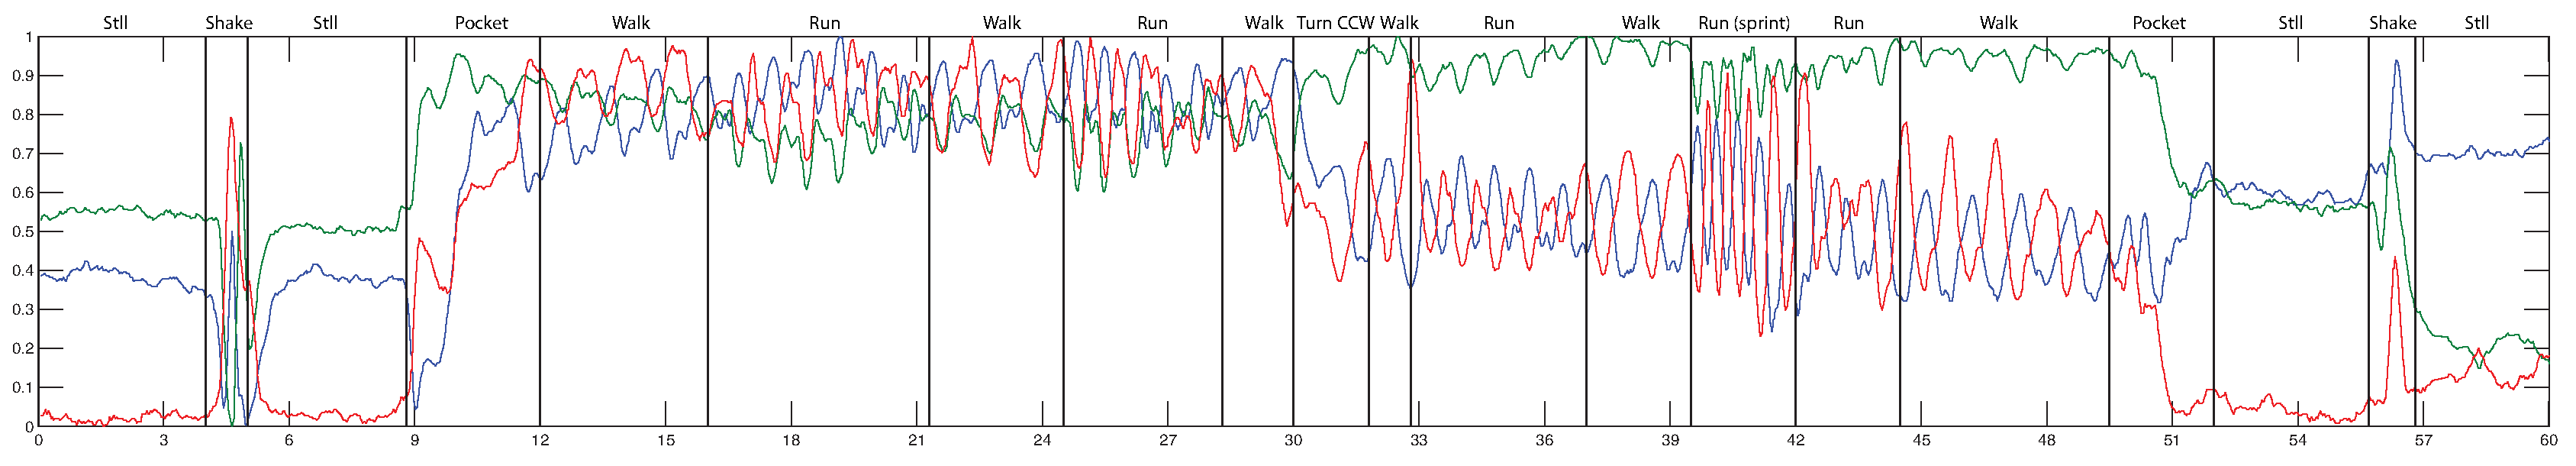
\includegraphics[width=1\textwidth]{./Figures/chapter6/data_collection/run-2-walk-run-jos/data_plot_mag_annotated.eps}
  \caption[R2: mag]{Run 2: Walk-run-jos, Mag}
  \label{fig:data_gathering_run_2_mag}
\end{figure}

\begin{figure}
\centering
  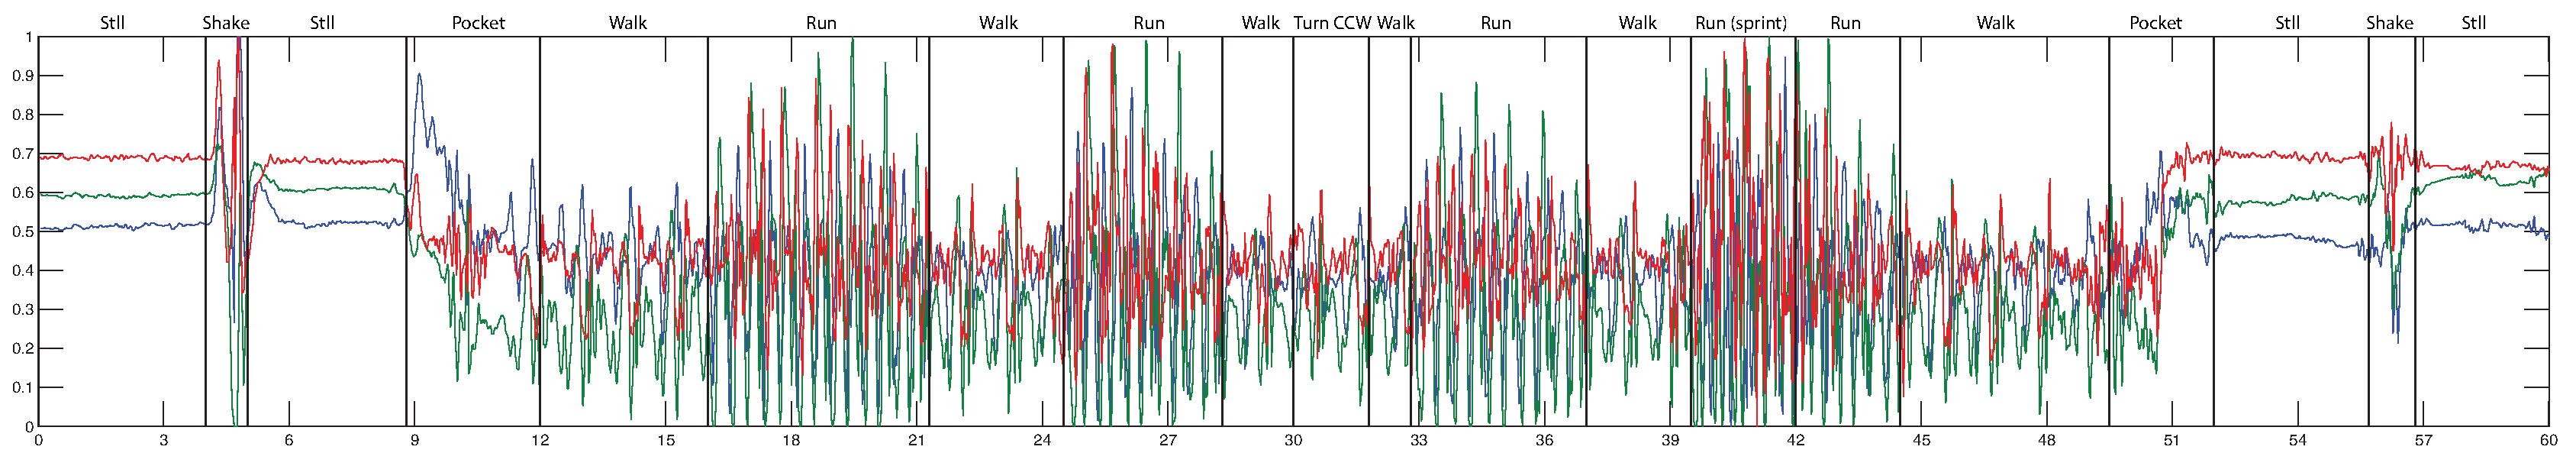
\includegraphics[width=1\textwidth]{./Figures/chapter6/data_collection/run-2-walk-run-jos/data_plot_acc_annotated.eps}
  \caption[R2: accelerometer]{Run 2: Walk-run-jos, accelerometer}
  \label{fig:data_gathering_run_2_ann}
\end{figure}

%---- Run 3: Stairs remco
\begin{figure}
\centering
  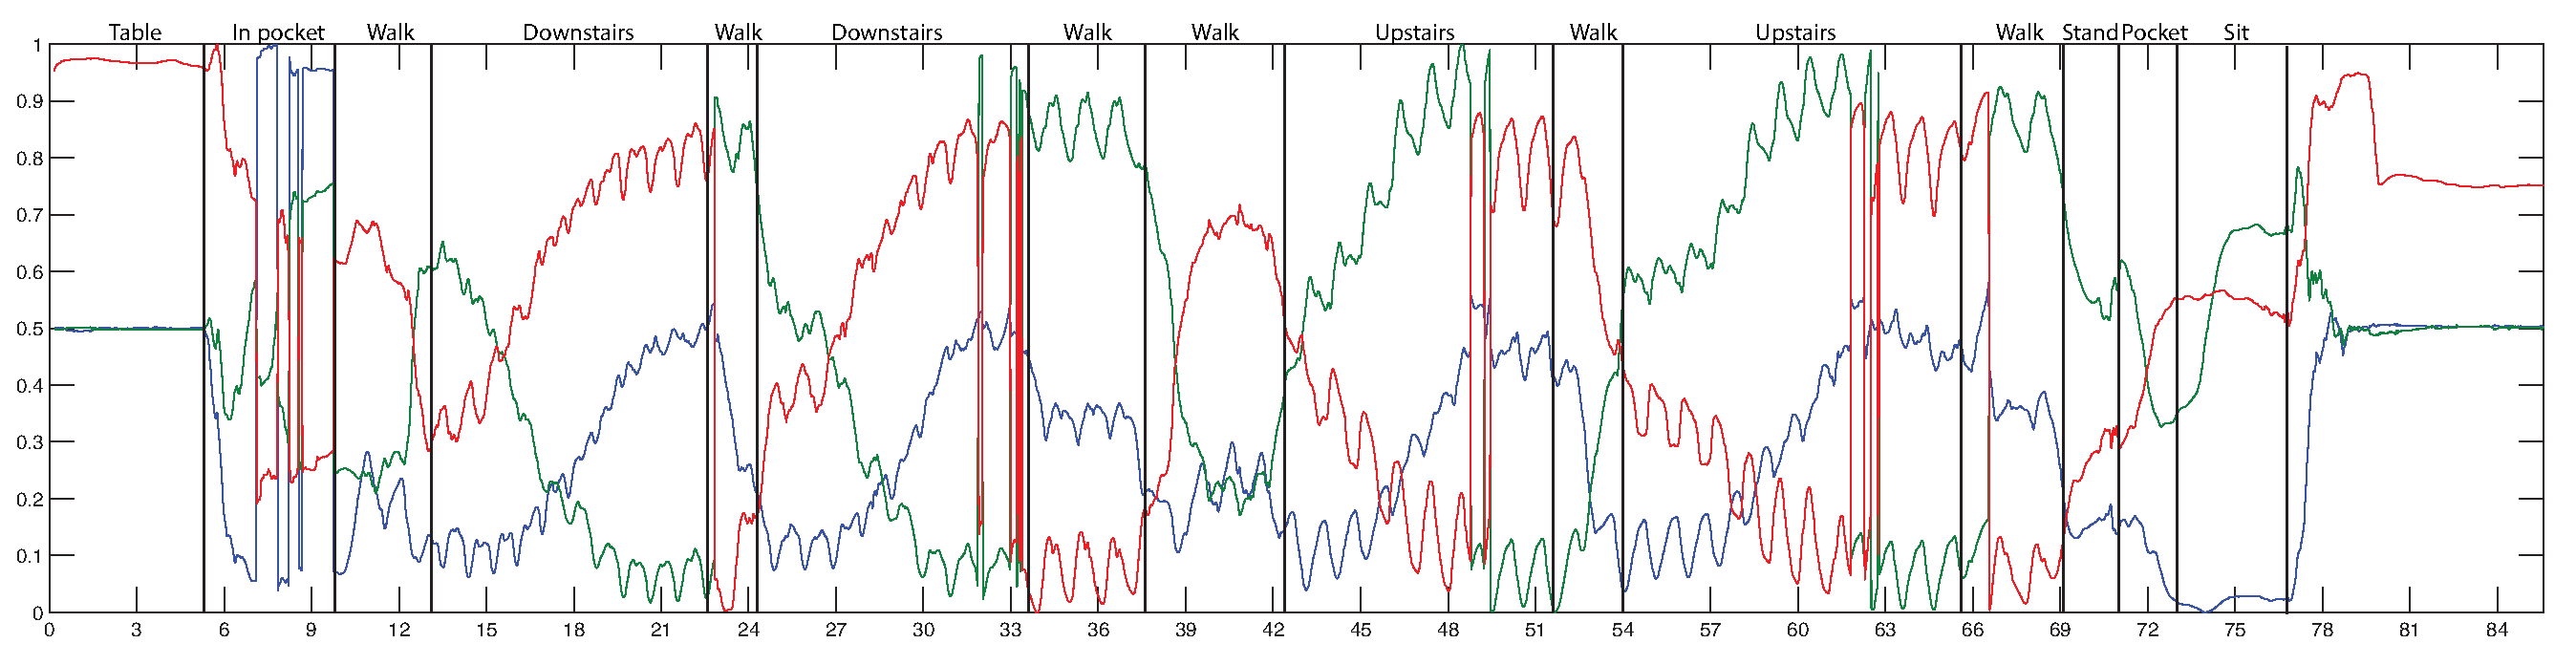
\includegraphics[width=1\textwidth]{./Figures/chapter6/data_collection/stairs-1-marc/data_plot_rot_annotated.eps}
  \caption[R3: rotation]{Run 3: Indoor stairs Marc, rotation}
  \label{fig:data_gathering_run_3_rot}
\end{figure}

\begin{figure}
\centering
  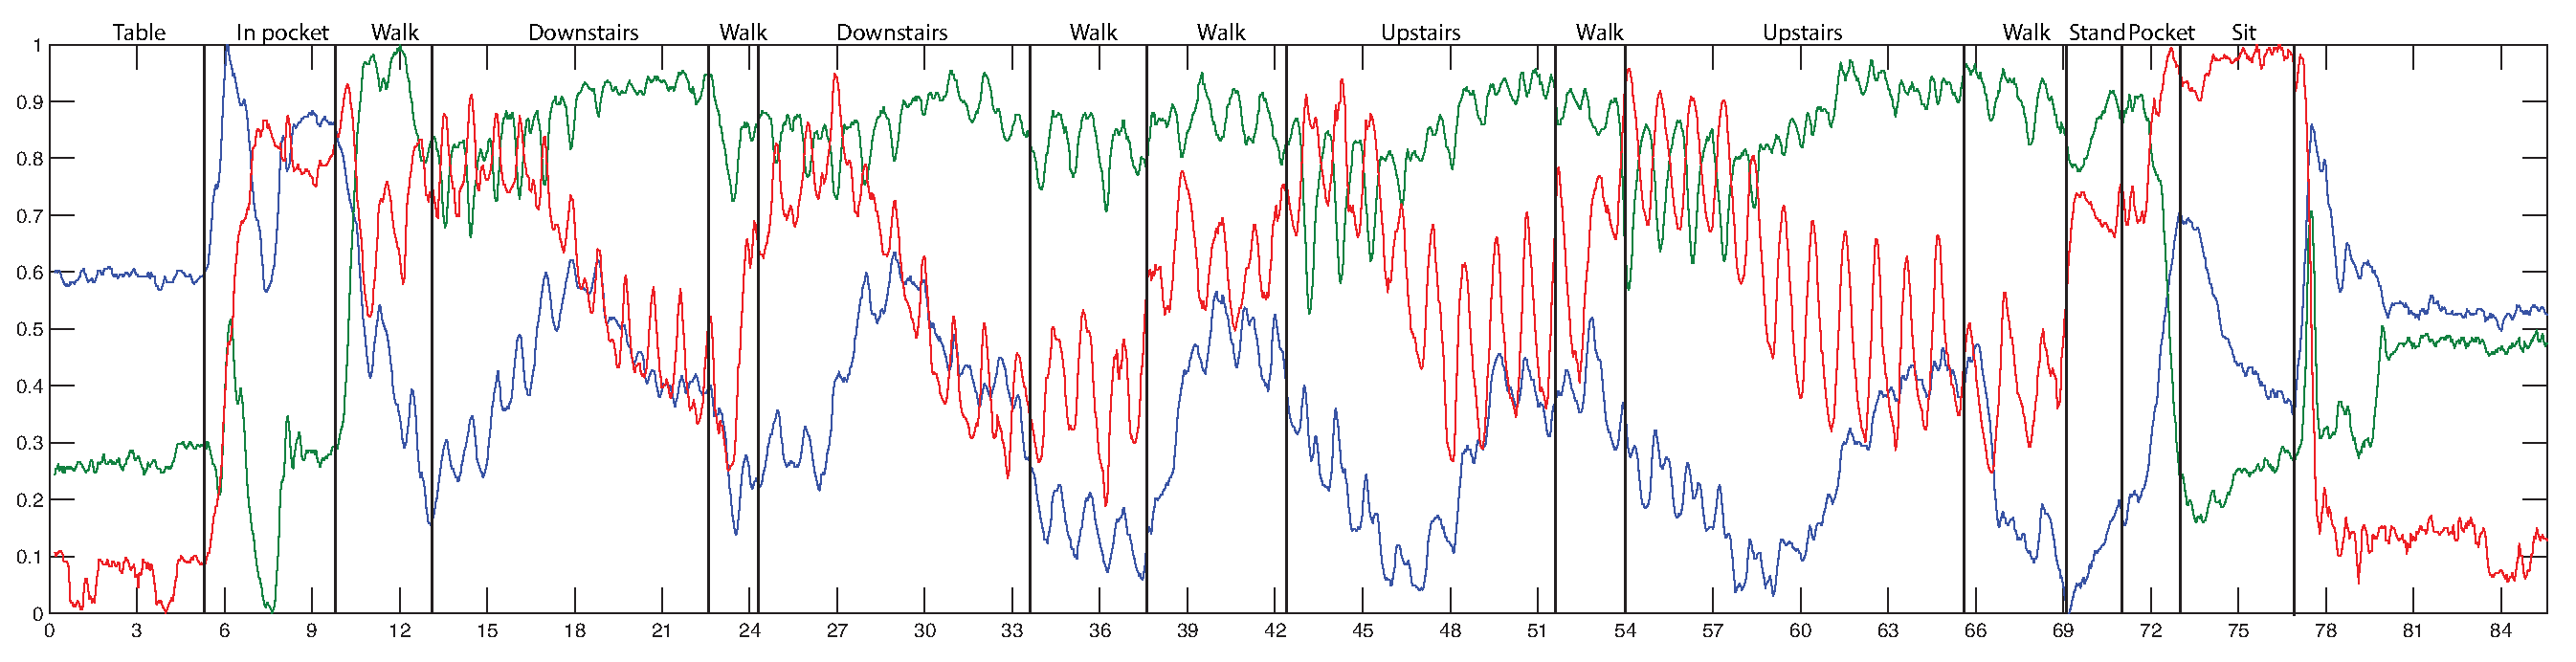
\includegraphics[width=1\textwidth]{./Figures/chapter6/data_collection/stairs-1-marc/data_plot_mag_annotated.eps}
  \caption[R3: mag]{Run 3: Indoor stairs Marc, Mag}
  \label{fig:data_gathering_run_3_mag}
\end{figure}

\begin{figure}
\centering
  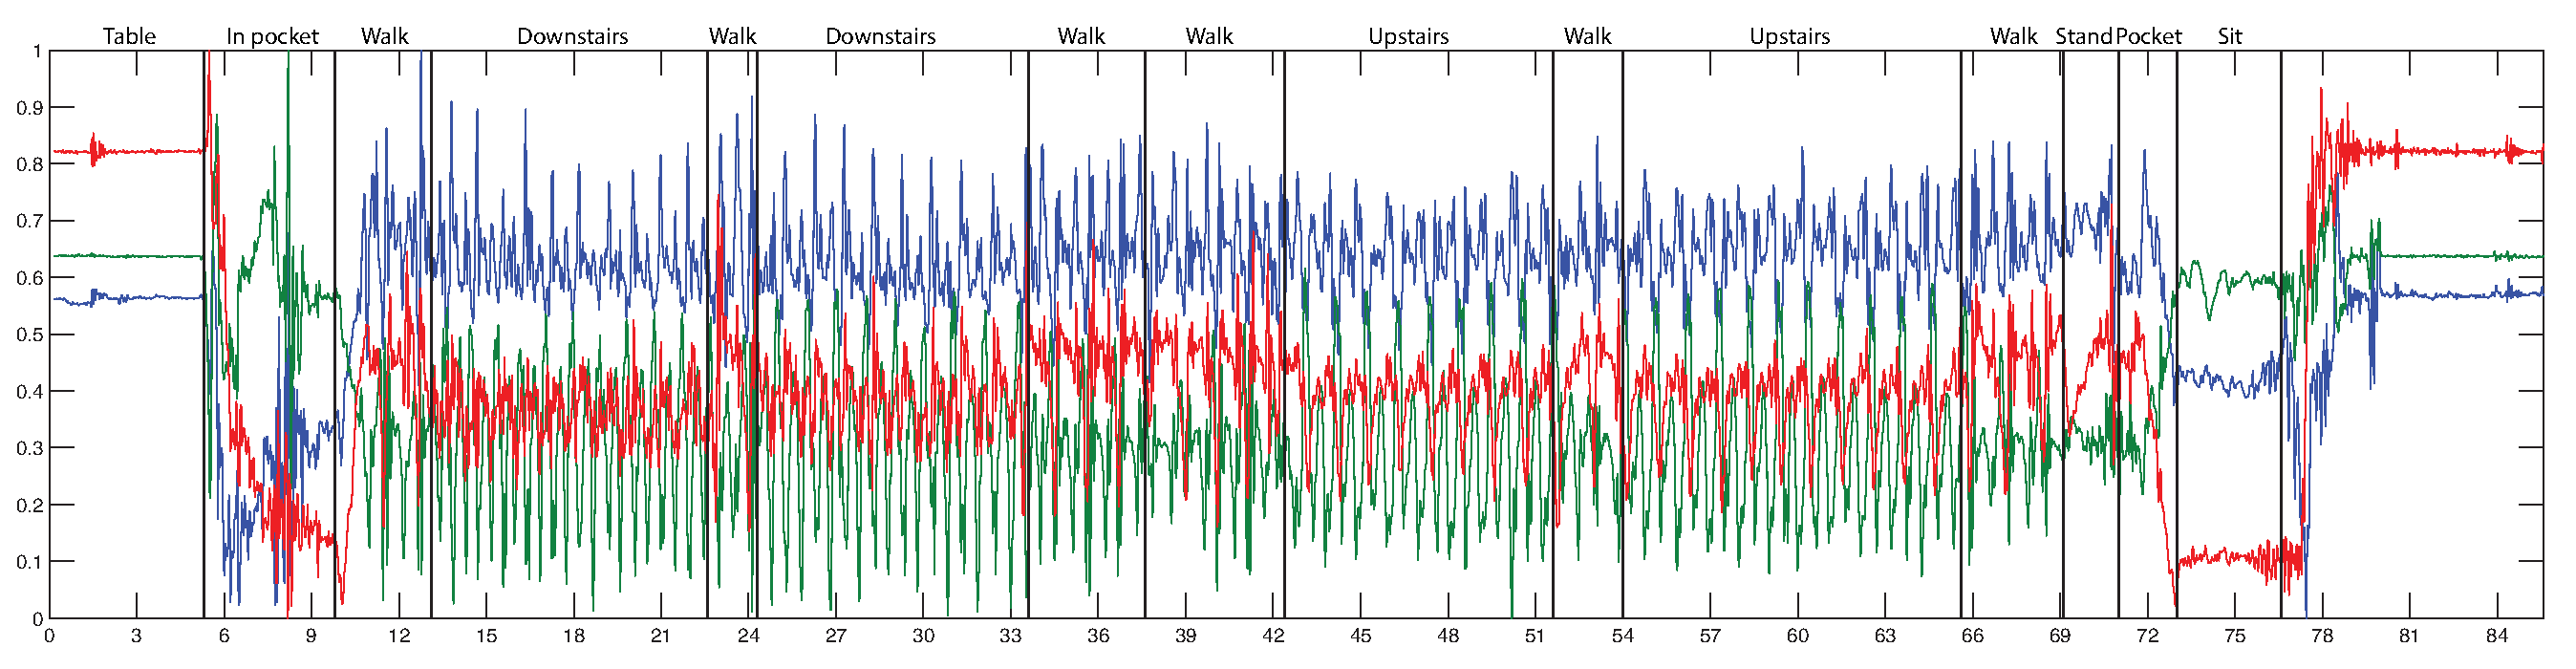
\includegraphics[width=1\textwidth]{./Figures/chapter6/data_collection/stairs-1-marc/data_plot_acc_annotated.eps}
  \caption[R3: accelerometer]{Run 3: Indoor stairs Marc, accelerometer}
  \label{fig:data_gathering_run_3_ann}
\end{figure}

\TODO{Add stills from video recordings, showing the kind of activities performed.}

Stills from subject 3:

\begin{figure}
\centering
  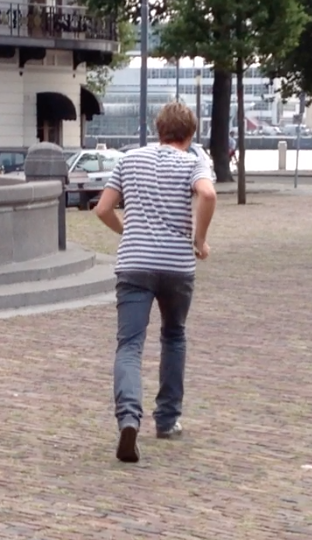
\includegraphics[width=1\textwidth]{./Figures/chapter6/data_collection/stills/jos_cp_walk-run.png}
  \caption[Recording still 1]{Subject 1 on the transition from walking to running}
  \label{fig:data_gathering_still_1_still_walk_to_run}
\end{figure}

\begin{figure}
\centering
  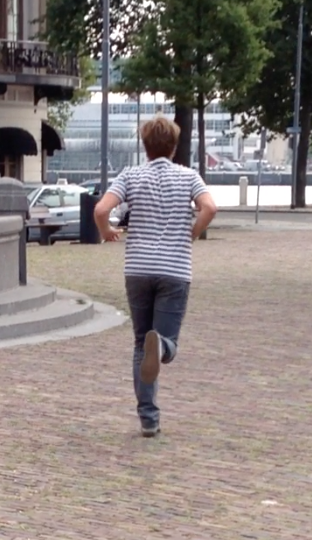
\includegraphics[width=1\textwidth]{./Figures/chapter6/data_collection/stills/jos_run_2.png}
  \caption[Recording still 2]{Subject 1 running}
  \label{fig:data_gathering_still_1_running}
\end{figure}

\begin{figure}
\centering
  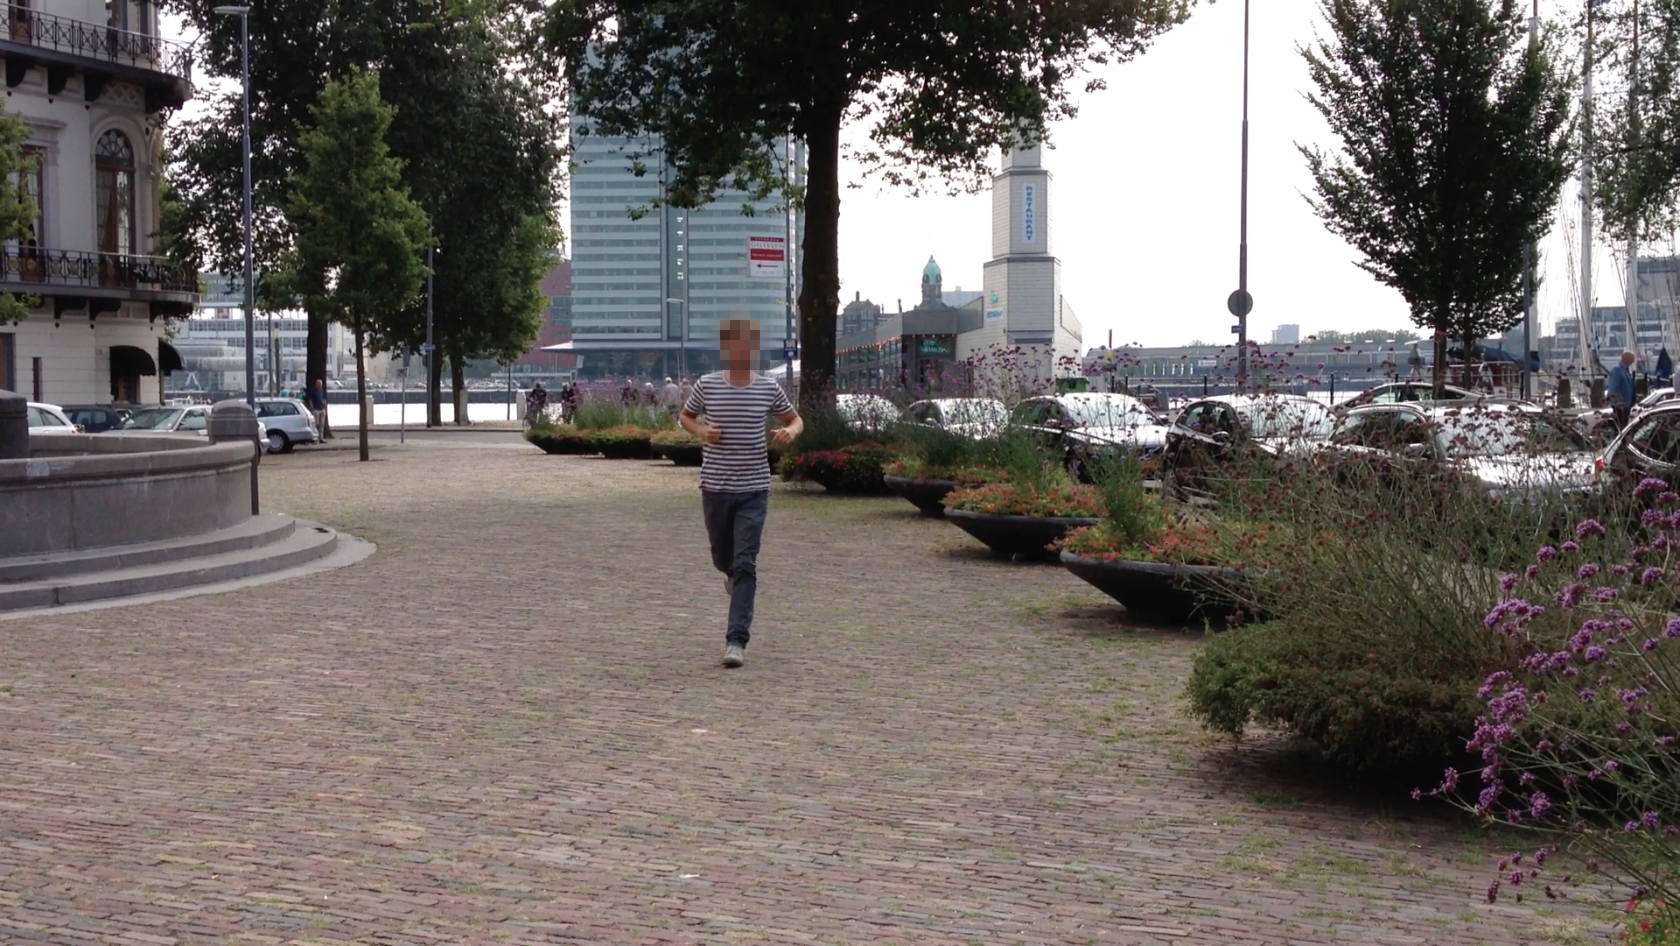
\includegraphics[width=1\textwidth]{./Figures/chapter6/data_collection/stills/jos_run.png}
  \caption[Recording still 3]{Subject 1 running}
  \label{fig:data_gathering_still_1_running_2}
\end{figure}

\begin{figure}
\centering
  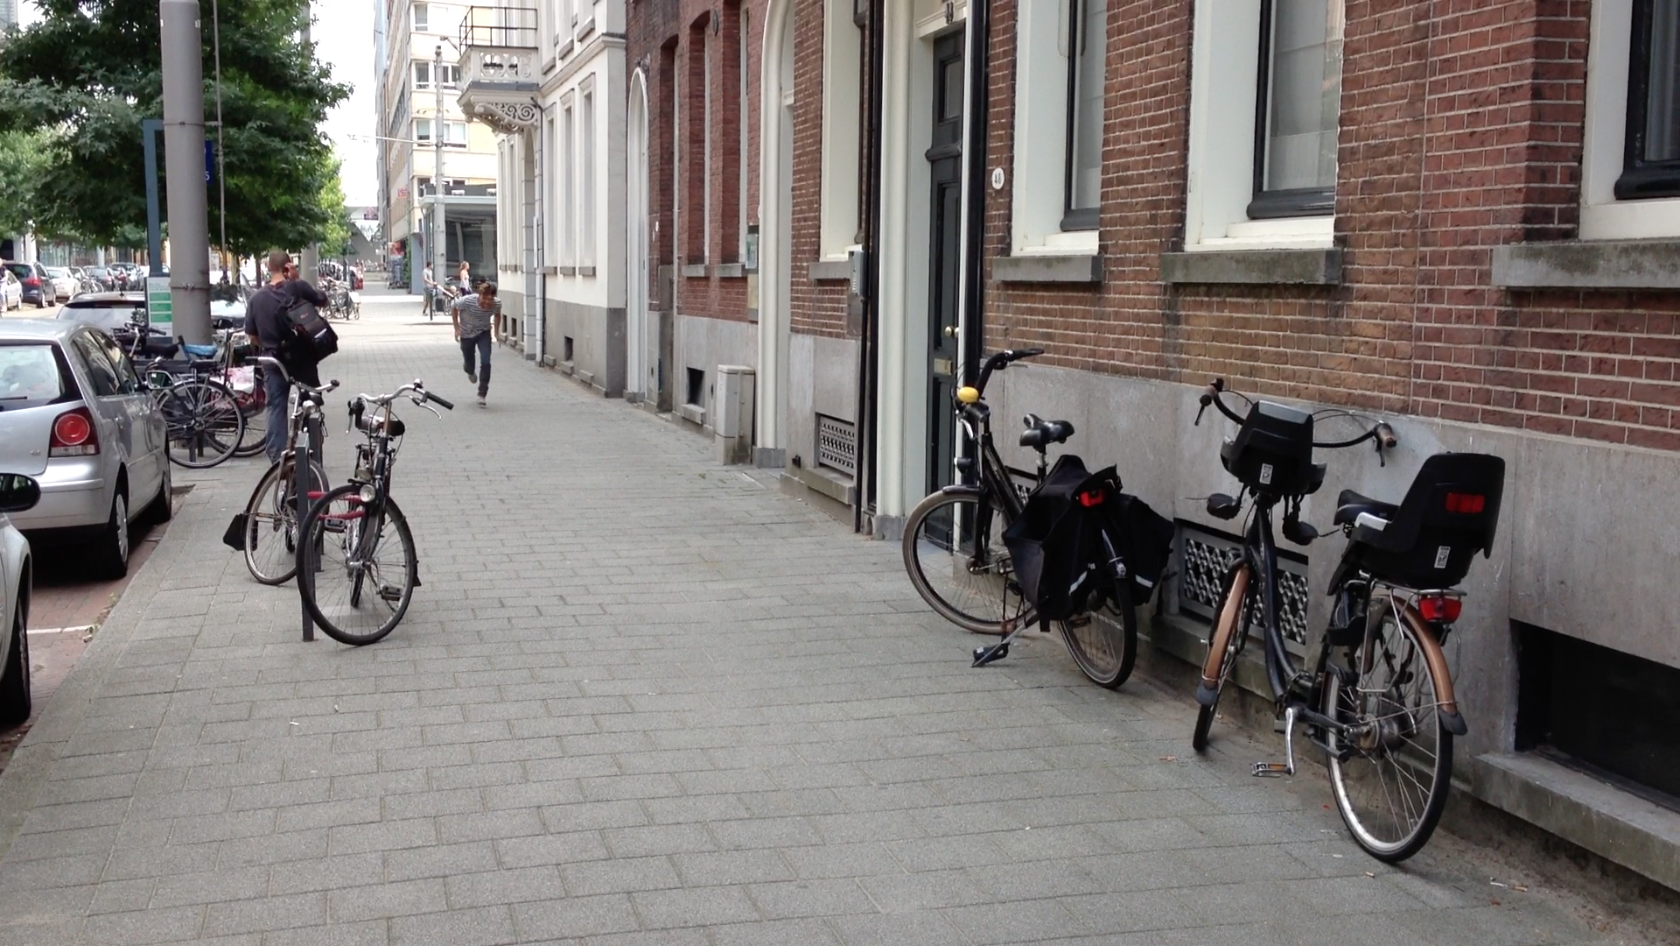
\includegraphics[width=1\textwidth]{./Figures/chapter6/data_collection/stills/jos_sprint.png}
  \caption[Recording still 4]{Subject 1 sprinting}
  \label{fig:data_gathering_still_1_sprint}
\end{figure}

\begin{figure}
\centering
  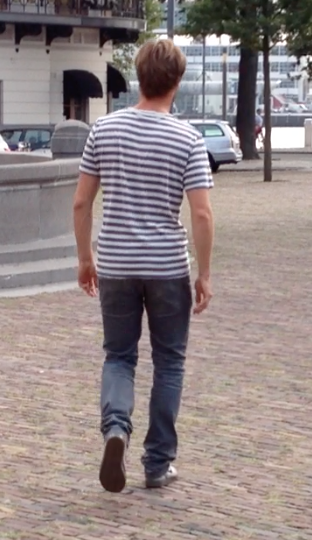
\includegraphics[width=1\textwidth]{./Figures/chapter6/data_collection/stills/jos_walking.png}
  \caption[Recording still 5]{Subject 1 walking}
  \label{fig:data_gathering_still_1_walk}
\end{figure}

Stills from subject 2:

\begin{figure}
\centering
  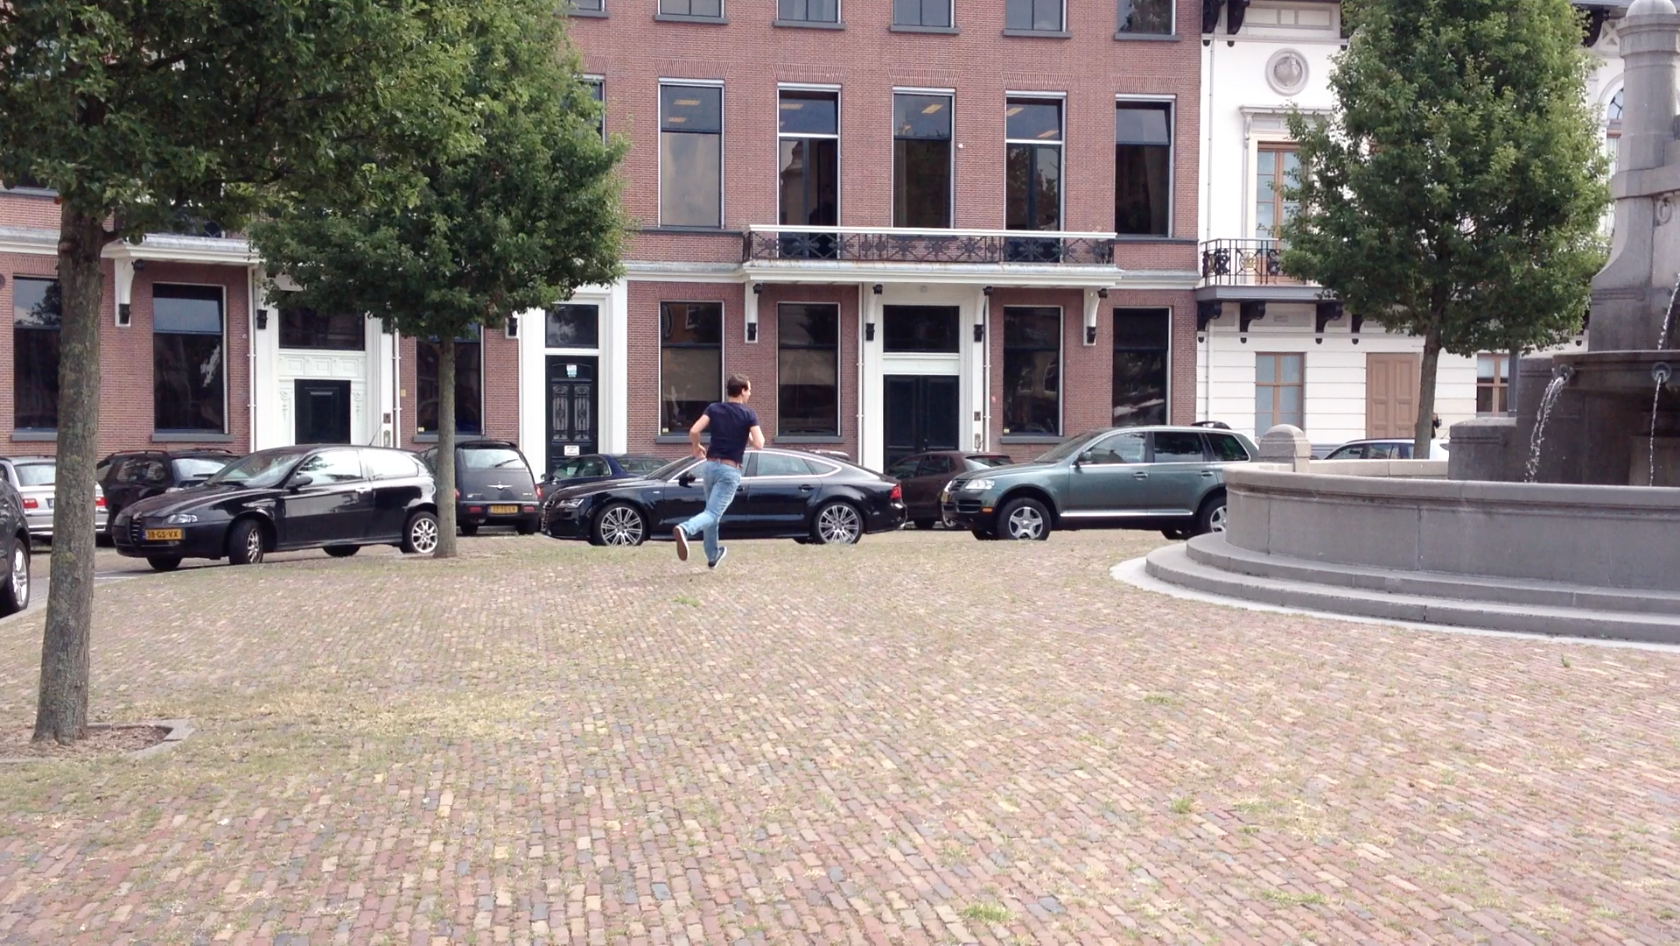
\includegraphics[width=1\textwidth]{./Figures/chapter6/data_collection/stills/roemer_run_cw.png}
  \caption[Recording still 6]{Subject 2 running in clockwise corner}
  \label{fig:data_gathering_still_2_run}
\end{figure}

\begin{figure}
\centering
  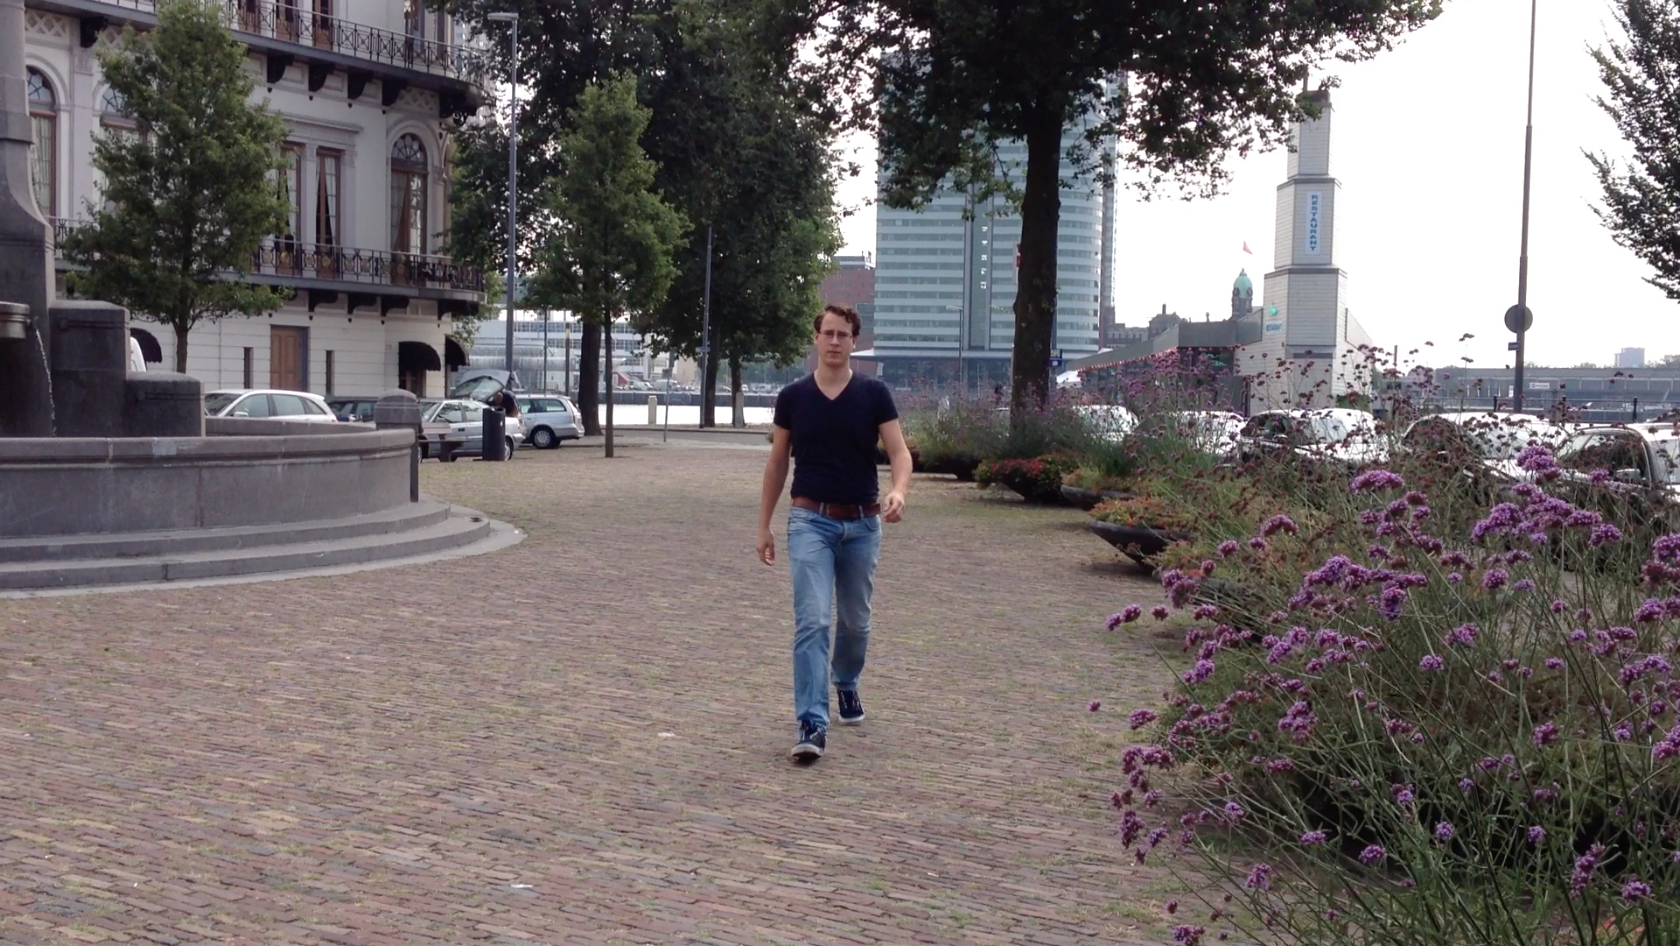
\includegraphics[width=1\textwidth]{./Figures/chapter6/data_collection/stills/roemer_walk.png}
  \caption[Recording still 7]{Subject 2 walking}
  \label{fig:data_gathering_still_2_walk}
\end{figure}

Stills from subject 3:

\begin{figure}
\centering
  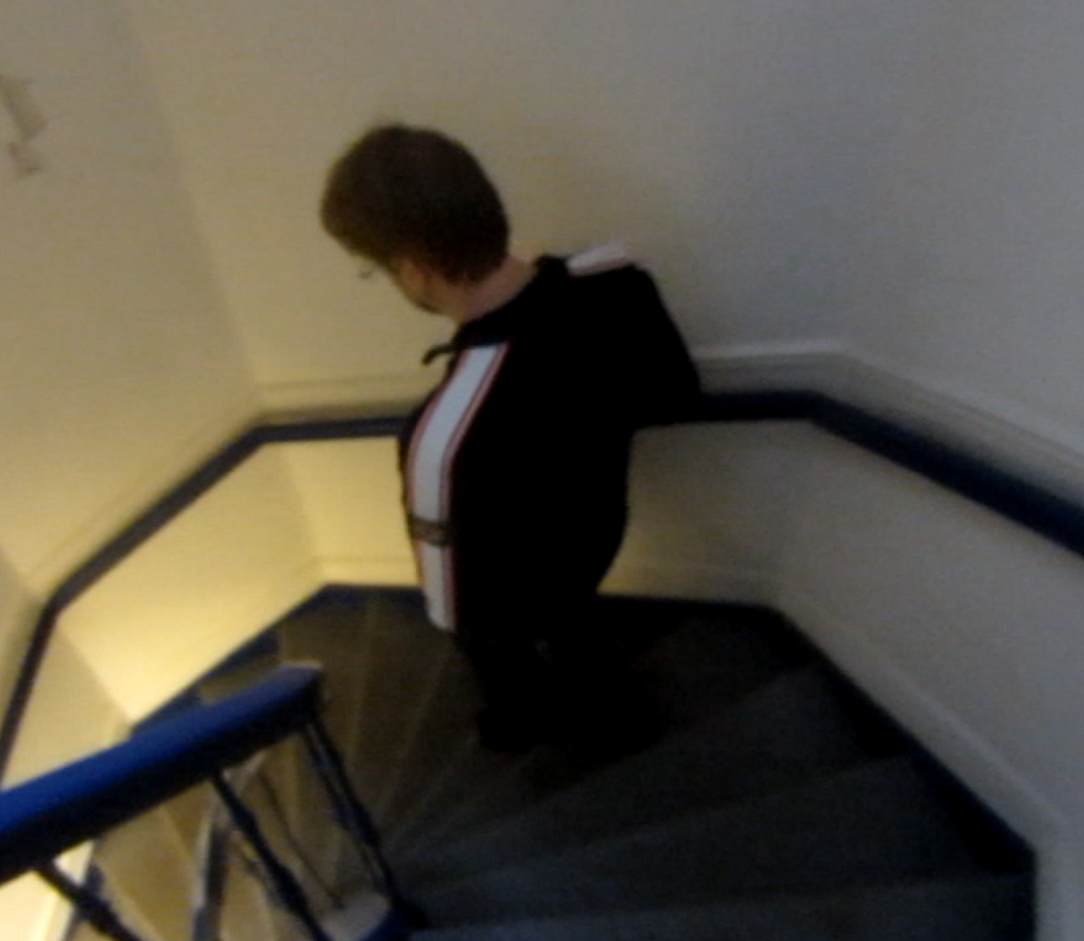
\includegraphics[width=1\textwidth]{./Figures/chapter6/data_collection/stills/marc_downstairs.png}
  \caption[Recording still 8]{Subject 3 descencing the stairs.}
  \label{fig:data_gathering_still_3_descending}
\end{figure}

\begin{figure}
\centering
  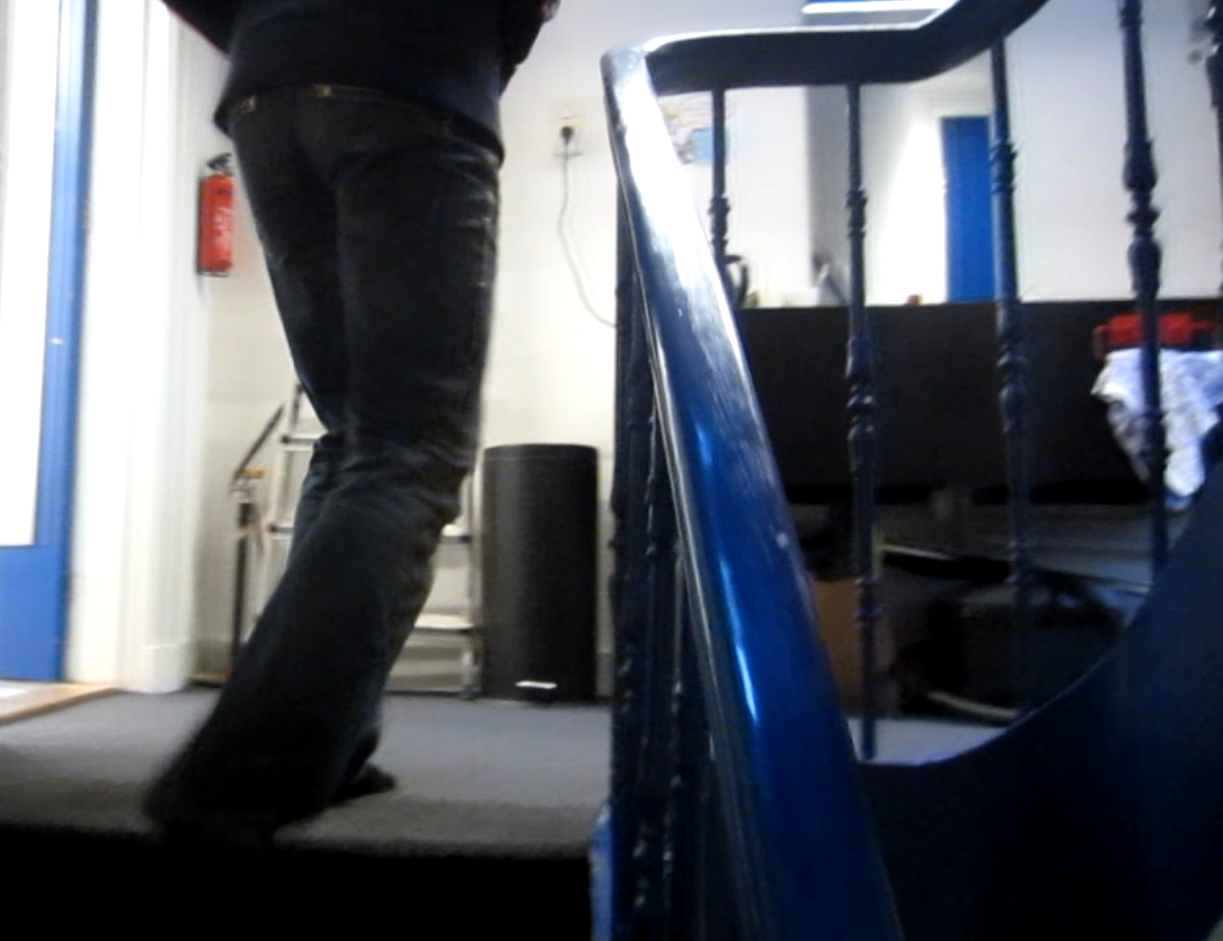
\includegraphics[width=1\textwidth]{./Figures/chapter6/data_collection/stills/marc_stairs_up_walk.png}
  \caption[Recording still 9]{Subject 3 will start walking for a small fragment and will continue ascending the stairs.}
  \label{fig:data_gathering_still_3_ascending}
\end{figure}

\begin{figure}
\centering
  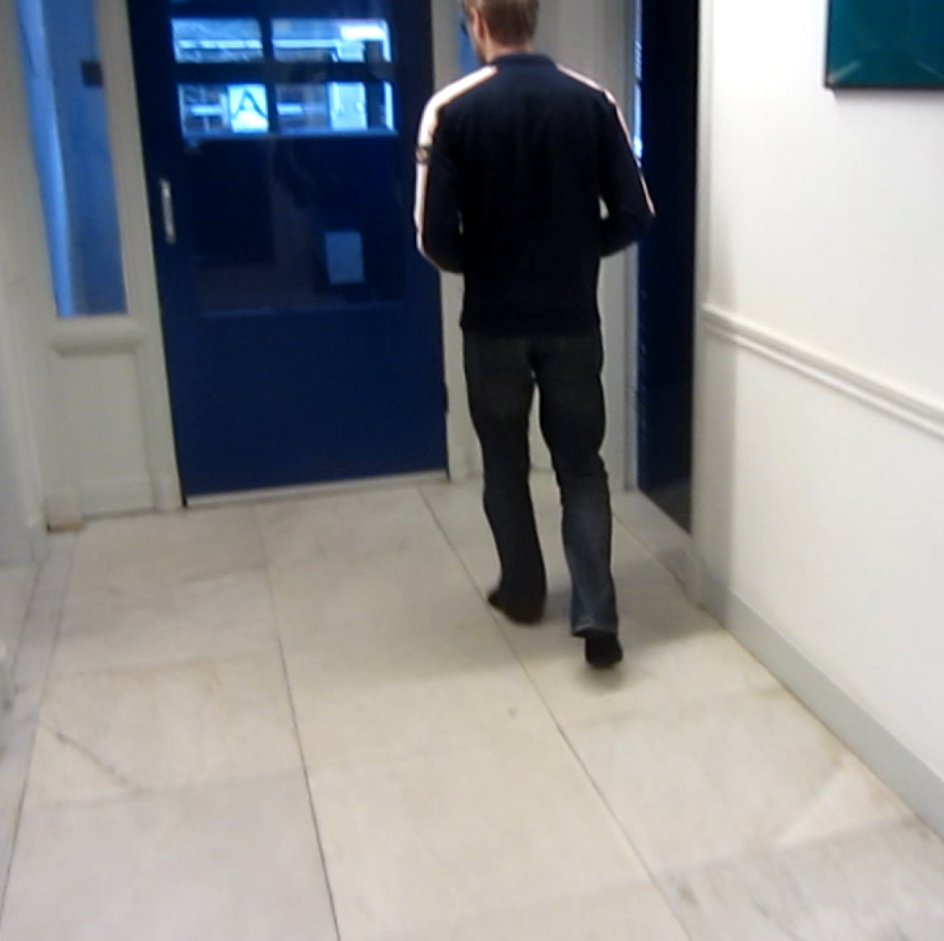
\includegraphics[width=1\textwidth]{./Figures/chapter6/data_collection/stills/marc_walk.png}
  \caption[Recording still 10]{Subject 3 walking in the hallway. He will turn $180^{\circ}$ counter-clockwise.}
  \label{fig:data_gathering_still_3_walk}
\end{figure}